\documentclass[10pt,letterpaper]{article}
\usepackage[margin=0.78in]{geometry}
\usepackage{amsmath,amssymb,booktabs,graphicx,array,float}
\usepackage[T1]{fontenc}
\usepackage{lmodern}
\usepackage{hyperref}
\hypersetup{colorlinks=true,linkcolor=blue,urlcolor=blue}
\setlength{\parindent}{0pt}
\setlength{\parskip}{5pt}
\title{Real-Trace Offline Evaluation of Budget-Constrained Selective Runtime Monitoring}
\author{CS 6158 Project: Shiyun Cheng and Gengkun Shao}
\date{October 18, 2026}
\begin{document}
\maketitle
\vspace{-1em}
\begin{abstract}
We evaluate five budgeted monitor-selection strategies using historical TraceMOP-derived data from two Java projects. Candidate groups, recorded trace identifiers, frequencies, and event-check cost proxies originate from an experimental workbook. At a 20\% proxy budget, utility-per-cost and redundancy-aware greedy both cover 97.8\% of observed unique trace IDs for \texttt{javadbf} and 99.7\% for \texttt{jlemmagen}. These are \emph{offline observed-trace coverage} measurements, not deployed monitoring recall, violation recall, or measured runtime savings.
\end{abstract}
\section{Research question and scope}
Our original project asks whether historical information about monitoring cost, usefulness, and redundancy can allocate a limited monitoring budget more effectively than simple baselines or Valg, particularly at comparable \emph{realized} overhead. This experiment addresses one intermediate question: how much of the previously observed distinct trace information could candidate subsets cover under a budget based on an event-check cost proxy? It does not yet test independently disabled/enabled creation-site monitors or compare against Valg's adaptive online policy.
\section{Dataset and preprocessing}
We use the \texttt{Monitor profile} worksheet of \texttt{valg-algorithm-input.xlsx}. Each worksheet row is treated as one candidate \emph{location $\times$ monitoring specification group}. The purported creation location is inferred from the first trace event, so it is not verified as an actual instrumentable creation site. Each candidate $i$ has a recorded frequency $f_i$, a positive cost proxy $c_i$ (\texttt{cost\_proxy\_event\_checks}), and a set $T_i$ of distinct recorded trace identifiers parsed from \texttt{trace\_ids}. Trace identifiers are unioned within each project; duplication across groups is counted once in coverage.

\begin{center}
\begin{tabular}{lrrr}\toprule
Project & Candidate groups & Observed distinct trace IDs & Total cost proxy \\\midrule
\texttt{javadbf} & 153 & 278 & 713,840 \\
\texttt{jlemmagen} & 66 & 2,115 & 8,572,328 \\\bottomrule
\end{tabular}
\end{center}

For project $p$, let $U_p=\bigcup_i T_i$ and $C_p=\sum_i c_i$. For each budget fraction $\beta\in\{0.10,0.20,0.30,0.50,0.80\}$, we select $S$ satisfying $\sum_{i\in S}c_i\leq\beta C_p$. Our outcome measure is
\[
\operatorname{ObservedTraceRecall}(S)=\frac{\left|\bigcup_{i\in S}T_i\right|}{|U_p|}.
\]
This denominator contains only trace IDs already present in the workbook: it is not the universe of all feasible execution traces. The proxy budget is in event-check units, \emph{not milliseconds, memory bytes, or realized total monitoring overhead}.
\section{Algorithms and reproducible protocol}
We compare (1) \textbf{Random}, shuffle candidates and include each item that fits; (2) \textbf{Frequency}, rank by $f_i$; (3) \textbf{Utility/cost}, rank by $|T_i|/c_i$; (4) \textbf{Redundancy-aware greedy}, repeatedly choose the affordable candidate maximizing $|T_i\setminus\bigcup_{j\in S}T_j|/c_i$, stopping when no positive marginal coverage fits; and (5) \textbf{Additive knapsack}, run discrete 0--1 knapsack maximizing $\sum_{i\in S}|T_i|$, with costs rounded upward for budget feasibility. Knapsack's internal objective \emph{double-counts overlapping trace IDs}; final recall is always computed by the union.

Each deterministic method is run once for each project--budget pair. Random is repeated 30 times per pair, using seeds 42--71; reported random results are means and sample standard deviations of \emph{selection variability on the same data}, not cross-program or timing uncertainty. All methods recompute a selection independently for each budget, rather than forcing larger-budget selections to contain smaller-budget selections. The executable implementation is \texttt{run\_experiments.py}; outputs include per-trial metrics, aggregate metrics, selections, and plots.
\section{Results}
\begin{table}[H]\centering\small
\caption{Observed unique-trace recall (\%) by budget. Random entries are mean $\pm$ SD over 30 trials.}
\begin{tabular}{llrrrrr}\toprule
Project & Budget & Random & Frequency & Utility/cost & Redundancy greedy & Additive knapsack \\\midrule
\texttt{javadbf} & 10\% & 89.6$\pm$0.0 & 89.6 & 89.6 & 89.6 & 70.5 \\
 & 20\% & 86.5$\pm$14.2 & 45.0 & 97.8 & 97.8 & 89.6 \\
 & 30\% & 90.7$\pm$2.6 & 11.2 & 97.8 & 97.8 & 96.8 \\
 & 50\% & 85.2$\pm$15.5 & 89.2 & 98.9 & 98.9 & 98.9 \\
 & 80\% & 99.1$\pm$1.6 & 99.6 & 99.6 & 99.6 & 99.3 \\\midrule
\texttt{jlemmagen} & 10\% & 43.1$\pm$38.9 & 88.4 & 99.5 & 99.5 & 99.3 \\
 & 20\% & 65.6$\pm$38.0 & 88.8 & 99.7 & 99.7 & 99.6 \\
 & 30\% & 64.0$\pm$39.0 & 1.8 & 99.8 & 99.8 & 99.7 \\
 & 50\% & 82.4$\pm$32.3 & 70.9 & 99.9 & 99.9 & 99.8 \\
 & 80\% & 90.2$\pm$24.5 & 99.8 & 100.0 & 100.0 & 99.9 \\\bottomrule
\end{tabular}
\end{table}
\begin{figure}[H]\centering
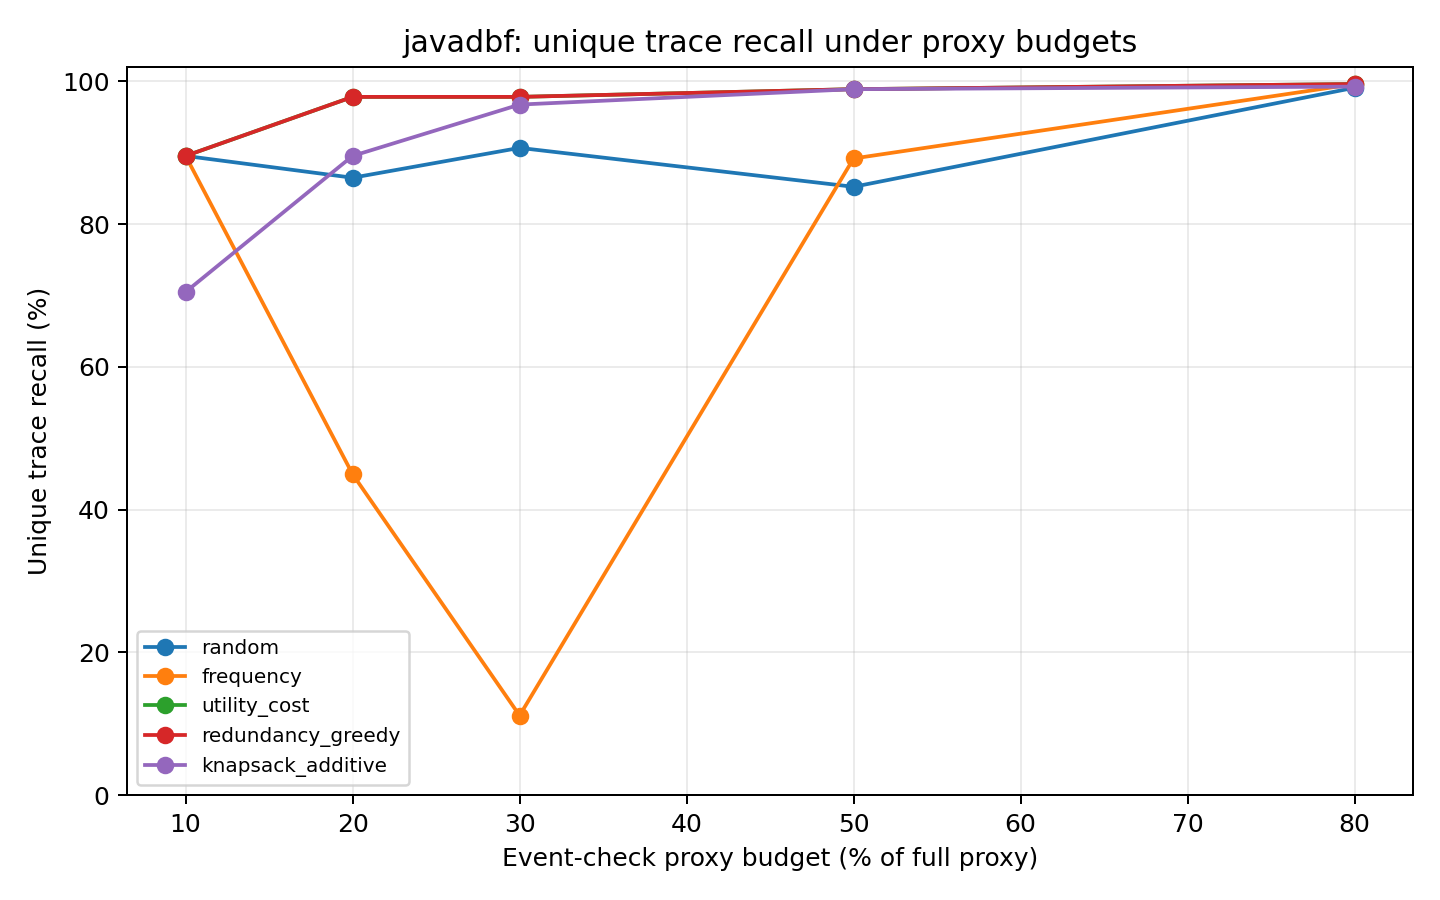
\includegraphics[width=.49\textwidth]{../results/offline/javadbf_trace_recall.png}\hfill
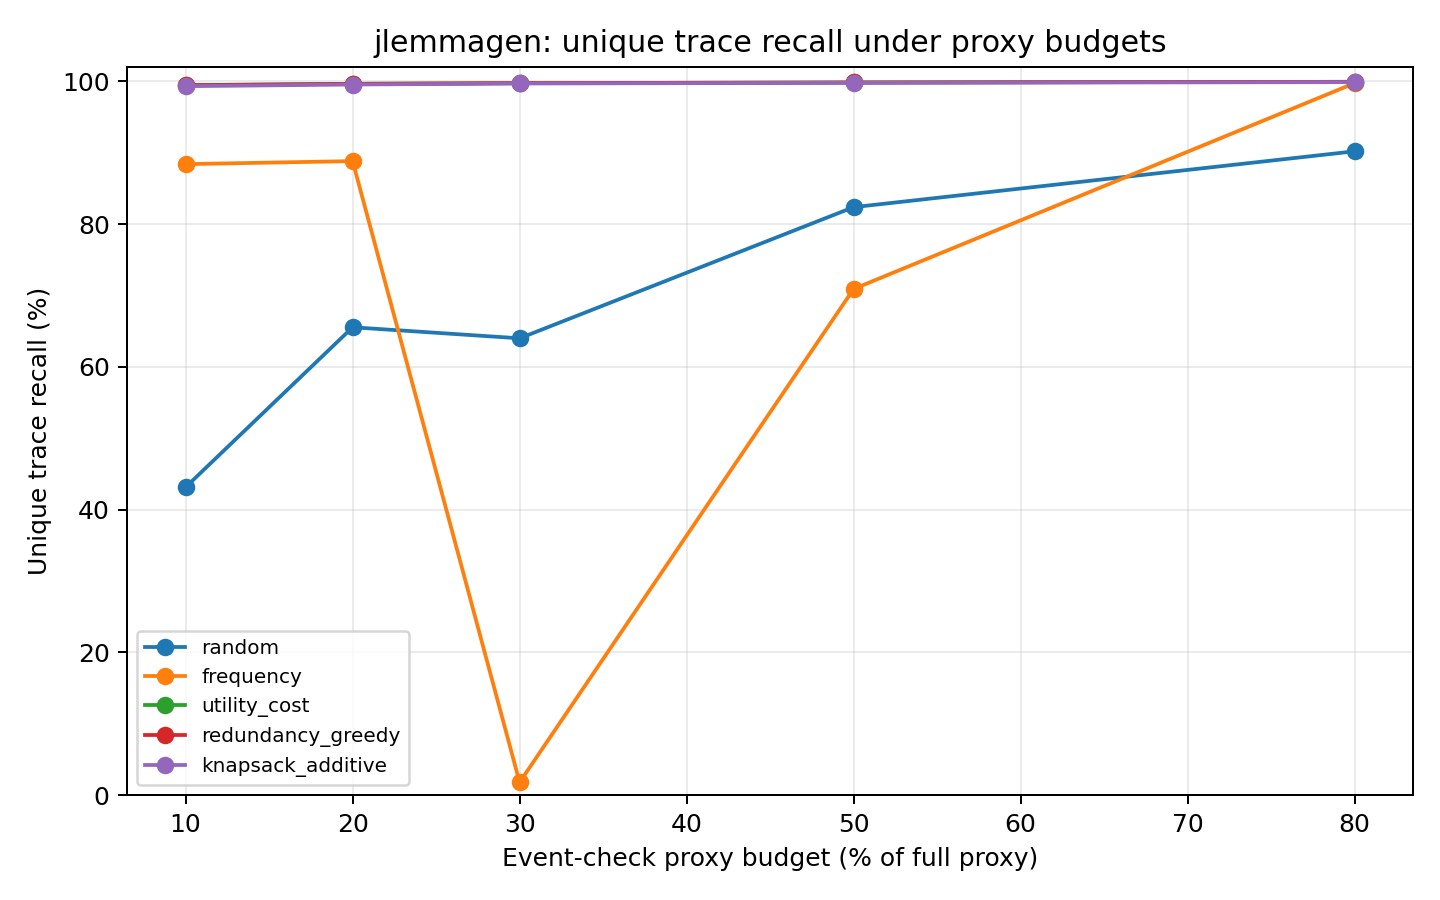
\includegraphics[width=.49\textwidth]{../results/offline/jlemmagen_trace_recall.png}
\caption{Coverage of historical trace IDs vs. percent of full event-check proxy budget. Curves are not empirical runtime--recall tradeoffs.}
\end{figure}
\textbf{Interpretation.} At 20\%, both utility/cost and redundancy-aware greedy obtain 97.8\% for \texttt{javadbf} and 99.7\% for \texttt{jlemmagen}. Their near-identical performance here provides no evidence that overlap-aware greedy is superior to static utility/cost on these workloads. Additive knapsack can perform worse because it optimizes a sum of standalone trace counts and rewards duplicate coverage multiple times. For example, its \texttt{javadbf} recall is 89.6\% at 20\%, below both coverage-aware methods.

The \emph{non-monotonic} frequency curve is not necessarily a data or coding error: at every new budget, a fixed ordered list is rescanned with a fit-or-skip rule. A larger budget may now admit a costly group early in that list, leaving insufficient budget for many inexpensive groups that were previously selected; hence chosen sets are not nested. This is particularly visible at \texttt{jlemmagen}'s 30\% budget (1.8\% recall). The large random standard deviations on \texttt{jlemmagen} likewise suggest that coverage is concentrated in particular candidate groups. On \texttt{javadbf} at 10\%, almost all 153 groups fit and the random trials happen to produce identical recall; this reflects the highly skewed proxy-cost distribution, not robust performance across datasets.
\section{Limitations and next steps}
These results are descriptive, in-sample, and offline. There is no separation of historical profiling executions from held-out evaluation executions. The creation-site assumption is unverified, and aggregated group trace sets do not establish what would remain observable if those creation sites were independently disabled. No per-group violation-signature attribution is available, so we do not measure violation recall or violation-weighted utility. Proxy event-check totals cannot support claims about actual elapsed time, memory use, or matched-overhead superiority to Valg. Cost additivity is also unvalidated.

Next we will (i) validate candidate groups against actual monitor-creation locations; (ii) add per-site enable/disable controls and test trace/violation preservation on held-out runs; (iii) measure runtime and memory for complete selected configurations; (iv) compare all methods against Valg at \emph{matched realized cost}; and, if possible, (v) test profiles trained on one revision against later revisions and add an exploration budget. If independent control is infeasible, we will clearly label a fallback based on profiling proxies as an offline simulation rather than a full runtime evaluation.
\end{document}
